% RePressDB JSS submission manuscript
\documentclass[final,5p,times,twocolumn,authoryear]{elsarticle}

\usepackage{amsmath,amssymb,bm}
\usepackage{booktabs}
\usepackage{tabularx}
\usepackage{threeparttable}
\usepackage{multirow}
\usepackage{graphicx}
\usepackage{siunitx}
\usepackage{xurl}
\usepackage{microtype}
\usepackage{placeins}
\usepackage{float}
\usepackage{dblfloatfix}
\usepackage{cuted}
\usepackage{caption}
\usepackage{balance}
\usepackage[hidelinks]{hyperref}
\usepackage[nameinlink,noabbrev]{cleveref}

\journal{Journal of Systems and Software}
\biboptions{authoryear,round}
\graphicspath{{./}}
\setlength{\emergencystretch}{2em}
\setlength{\textfloatsep}{11pt plus 2pt minus 2pt}
\setlength{\floatsep}{9pt plus 2pt minus 2pt}
\raggedbottom
\sisetup{detect-all,group-separator={,},group-minimum-digits=4}
% Auto-generated from frozen CSV/JSON evidence. Do not edit manually.
\newcommand{\EvidenceFreezeVOneFiveOne}{19aad963a625e14c2298bb783bc4885dff062ae17427200f0f1cfbcb7713ed39}
\newcommand{\EvidenceFreezeVOneSevenZero}{ff773467a5de296e07dcbaac904b2d26c466a815ca7b16bdcddbff527a2c4088}
\newcommand{\ReplayRepressShapeRatio}{0.9617}
\newcommand{\ReplayRepressShapeLow}{0.9551}
\newcommand{\ReplayRepressShapeHigh}{0.9689}
\newcommand{\ReplayRepressShapeWins}{18}
\newcommand{\ReplayRepressInitialRatio}{0.9488}
\newcommand{\ReplayRepressInitialLow}{0.9365}
\newcommand{\ReplayRepressInitialHigh}{0.9609}
\newcommand{\ReplayRepressInitialWins}{18}
\newcommand{\ReplayRepressPHRatio}{0.9800}
\newcommand{\ReplayRepressPHLow}{0.9710}
\newcommand{\ReplayRepressPHHigh}{0.9888}
\newcommand{\ReplayRepressPHWins}{15}
\newcommand{\ReplayRepressAFHCRatio}{0.8780}
\newcommand{\ReplayRepressAFHCLow}{0.8439}
\newcommand{\ReplayRepressAFHCHigh}{0.9123}
\newcommand{\ReplayRepressAFHCWins}{18}
\newcommand{\ReplayRepressBestStaticRatio}{1.0564}
\newcommand{\ReplayRepressBestStaticLow}{1.0311}
\newcommand{\ReplayRepressBestStaticHigh}{1.0819}
\newcommand{\ReplayRepressBestStaticWins}{3}
\newcommand{\ReplayRepressMigrations}{185}
\newcommand{\ReplayShapeMigrations}{361}
\newcommand{\ReplayRepressUnamortized}{8.65\%}
\newcommand{\ReplayShapeUnamortized}{70.91\%}
\newcommand{\ReplayRepressStale}{12.43\%}
\newcommand{\ReplayShapeStale}{22.19\%}
\newcommand{\EndToEndQueries}{16,908,066}
\newcommand{\EndToEndPairs}{54}
\newcommand{\EndToEndWorkers}{108}
\newcommand{\EndToEndRepressShapeRatio}{0.9575}
\newcommand{\EndToEndRepressShapeLow}{0.7605}
\newcommand{\EndToEndRepressShapeHigh}{1.2027}
\newcommand{\EndToEndRepressShapeMedian}{1.0009}
\newcommand{\EndToEndRepressInitialRatio}{0.9896}
\newcommand{\EndToEndRepressInitialLow}{0.8379}
\newcommand{\EndToEndRepressInitialHigh}{1.1302}
\newcommand{\EndToEndRepressShapePnnRatio}{1.1256}
\newcommand{\EndToEndRepressShapePnnLow}{0.8470}
\newcommand{\EndToEndRepressShapePnnHigh}{1.5159}
\newcommand{\EndToEndRepressInitialPnnRatio}{1.3803}
\newcommand{\EndToEndRepressInitialPnnLow}{1.0653}
\newcommand{\EndToEndRepressInitialPnnHigh}{1.7535}
\newcommand{\LegacyDiagnosticRepressShape}{1.4142}
\newcommand{\CombinedRecoveryTrials}{1,100}
\newcommand{\CalibrationSeconds}{26.10}
\newcommand{\CalibrationReadMB}{923.23}
\newcommand{\CalibrationWriteMB}{113.15}
\newcommand{\CalibrationCandidateRatio}{3.94}
\newcommand{\CacheInitialServiceRatio}{0.4718}
\newcommand{\CacheInitialServiceLow}{0.3778}
\newcommand{\CacheInitialServiceHigh}{0.6084}
\newcommand{\CacheInitialDispatchRatio}{0.0329}
\newcommand{\CacheInitialPnnRatio}{0.4548}
\newcommand{\CacheShapeServiceRatio}{0.3560}
\newcommand{\CacheShapeServiceLow}{0.3400}
\newcommand{\CacheShapeServiceHigh}{0.3734}
\newcommand{\CacheShapeDispatchRatio}{0.0198}
\newcommand{\CacheShapePnnRatio}{0.3333}
\newcommand{\CacheRepressServiceRatio}{0.2638}
\newcommand{\CacheRepressServiceLow}{0.2168}
\newcommand{\CacheRepressServiceHigh}{0.3316}
\newcommand{\CacheRepressDispatchRatio}{0.0123}
\newcommand{\CacheRepressPnnRatio}{0.3761}

\input{artifact_links.tex}

\begin{document}

\begin{frontmatter}

\title{RePressDB: A Dependable Self-Adaptive Storage Architecture for Nonstationary Time-Series Workloads}

\author[aff1]{Zhichao Zhang\corref{cor1}}
\ead{zhichao.zhang2024@outlook.com}
\author[aff2]{Xiaolu Peng\fnref{equal2}}
\ead{lilypxl1656179423@outlook.com}
\author[aff1]{Daoqi Sun\fnref{equal2}}
\ead{sundao0217@gmail.com}
\cortext[cor1]{Corresponding author: Zhichao Zhang (zhichao.zhang2024@outlook.com).}
\fntext[equal2]{Xiaolu Peng and Daoqi Sun contributed equally to this work and are co-second authors.}
\address[aff1]{School of Science, Minzu University of China, No. 27 Zhongguancun South Avenue, Beijing, 100081, China}
\address[aff2]{School of Navigation, Dalian Maritime University, No. 1 Linghai Road, Ganjingzi District, Dalian 116026, China}

\begin{abstract}
Long-running time-series services experience shifts in query behavior, causing a physical representation that is efficient for one workload regime to lose efficiency as access patterns change. Changing the representation online consumes I/O, modifies durable state, and creates recovery obligations. We present RePressDB, a dependable self-adaptive storage architecture that coordinates workload monitoring, reconfiguration admission, and recoverable physical actuation. RePressDB combines dual-timescale query-shape monitoring with measured layout cost, a directed break-even test, confirmation, cooldown, and a global write budget. Accepted changes pass through a single-active transaction over versioned files and a SQLite WAL catalog, while a version-keyed active view keeps steady-state readers aligned with the published version. Across 18 continuous trace realizations, RePressDB achieves a measured-cost ratio of \ReplayRepressShapeRatio{} relative to Shape-EWMA-BE and reduces migrations from \ReplayShapeMigrations{} to \ReplayRepressMigrations. A paired file-backed campaign covering \EndToEndQueries{} verified queries gives a RePressDB/Shape-EWMA-BE service-time ratio of \EndToEndRepressShapeRatio, and the active view reduces catalog-dispatch time by 96.71--98.77\%. Across \CombinedRecoveryTrials{} controlled interruption and corruption trials, every completed trial recovers to a valid active-store state with correct query results. The evaluation shows that selective workload adaptation can reduce persistent reconfiguration activity while retaining competitive end-to-end service efficiency and an explicit recovery path.
\end{abstract}

\begin{keyword}
self-adaptive systems \sep storage architecture \sep runtime reconfiguration \sep workload drift \sep time-series storage \sep crash recovery \sep empirical software engineering
\end{keyword}

\end{frontmatter}

\section{Introduction}
\label{sec:introduction}

Long-running data services rarely operate under a fixed query mix. In time-series platforms, monitoring agents, dashboards, and analytical jobs shift the balance among point lookups, selective ranges, broad scans, and aggregates over time. These query classes favor different physical organizations, so a representation chosen at deployment can become increasingly expensive as the workload evolves.

Changing a physical layout at runtime has consequences beyond query latency. The system rewrites data, updates durable metadata, consumes I/O, and may leave recovery work after interruption. A useful adaptation policy must therefore consider both the persistence of the observed workload and the cost of the action it triggers. Frequent changes increase physical churn, while delayed changes prolong operation under a poorly matched layout. This coupling between adaptation decisions and durable state motivates an architectural treatment of online storage reconfiguration.

Several research areas address parts of this problem. Database physical-design techniques use workload evidence and cost models to select candidate structures \citep{chaudhuri1997autoadmin,bruno2005physical,vanaken2017ottertune,pavlo2017selfdriving}. Self-adaptive software provides feedback-loop structures for monitoring runtime change and selecting actions under uncertainty \citep{kephart2003vision,garlan2004rainbow,salehie2009landscape,delemos2013roadmap}. Compressed time-series systems demonstrate the performance consequences of representation choice \citep{pelkonen2015gorilla,andersen2016btrdb,blalock2018sprintz}. RePressDB addresses the point where these concerns meet: a runtime adaptation decision that can trigger an expensive persistent rewrite and must preserve a recoverable active representation.

We present RePressDB, a dependable self-adaptive storage architecture for nonstationary time-series workloads. The controller observes query shape at short and long time scales and admits a representation change after target agreement, repeated confirmation, a relative-gain threshold, and a directed break-even test. Cooldown regulates rapid reversals, and a global write budget limits aggregate rewrite activity. Accepted changes execute through a single-active transaction over versioned files and a SQLite WAL catalog, with recovery transitions defined around the same catalog commit that changes reader visibility.

The steady-state read path uses a version-keyed active view that binds the current catalog entry, parsed metadata, representation state, and open handles to the published version. Migration or recovery invalidates the view and causes the next query to resolve the new version. This keeps routine metadata work consistent with the cost model used by the controller and places adaptation, reconfiguration, publication, and recovery on one runtime control path (\cref{fig:architecture}).

The evaluation follows that control path. Across 18 continuous trace realizations, RePressDB reaches a measured-cost ratio of \ReplayRepressShapeRatio{} relative to Shape-EWMA-BE while reducing migrations from \ReplayShapeMigrations{} to \ReplayRepressMigrations. A paired file-backed campaign covering \EndToEndQueries{} verified queries yields a RePressDB/Shape-EWMA-BE service-time ratio of \EndToEndRepressShapeRatio. The recovery campaign exercises \CombinedRecoveryTrials{} controlled interruption and corruption scenarios, with every completed trial returning to a valid active-store state.

The paper makes three contributions.

\begin{enumerate}
    \item A self-adaptive storage architecture that combines workload persistence, measured layout cost, directed rewrite economics, and bounded write activity when admitting a physical-layout change.
    \item A dependable actuation path with single-active publication, versioned state, explicit recovery transitions, and a version-keyed active view that keeps reader state aligned with the published version.
    \item An empirical evaluation that links adaptation effectiveness under continuous nonstationarity to file-backed runtime behavior and recovery under controlled interruption and corruption.
\end{enumerate}

\begin{figure*}[t]
\centering
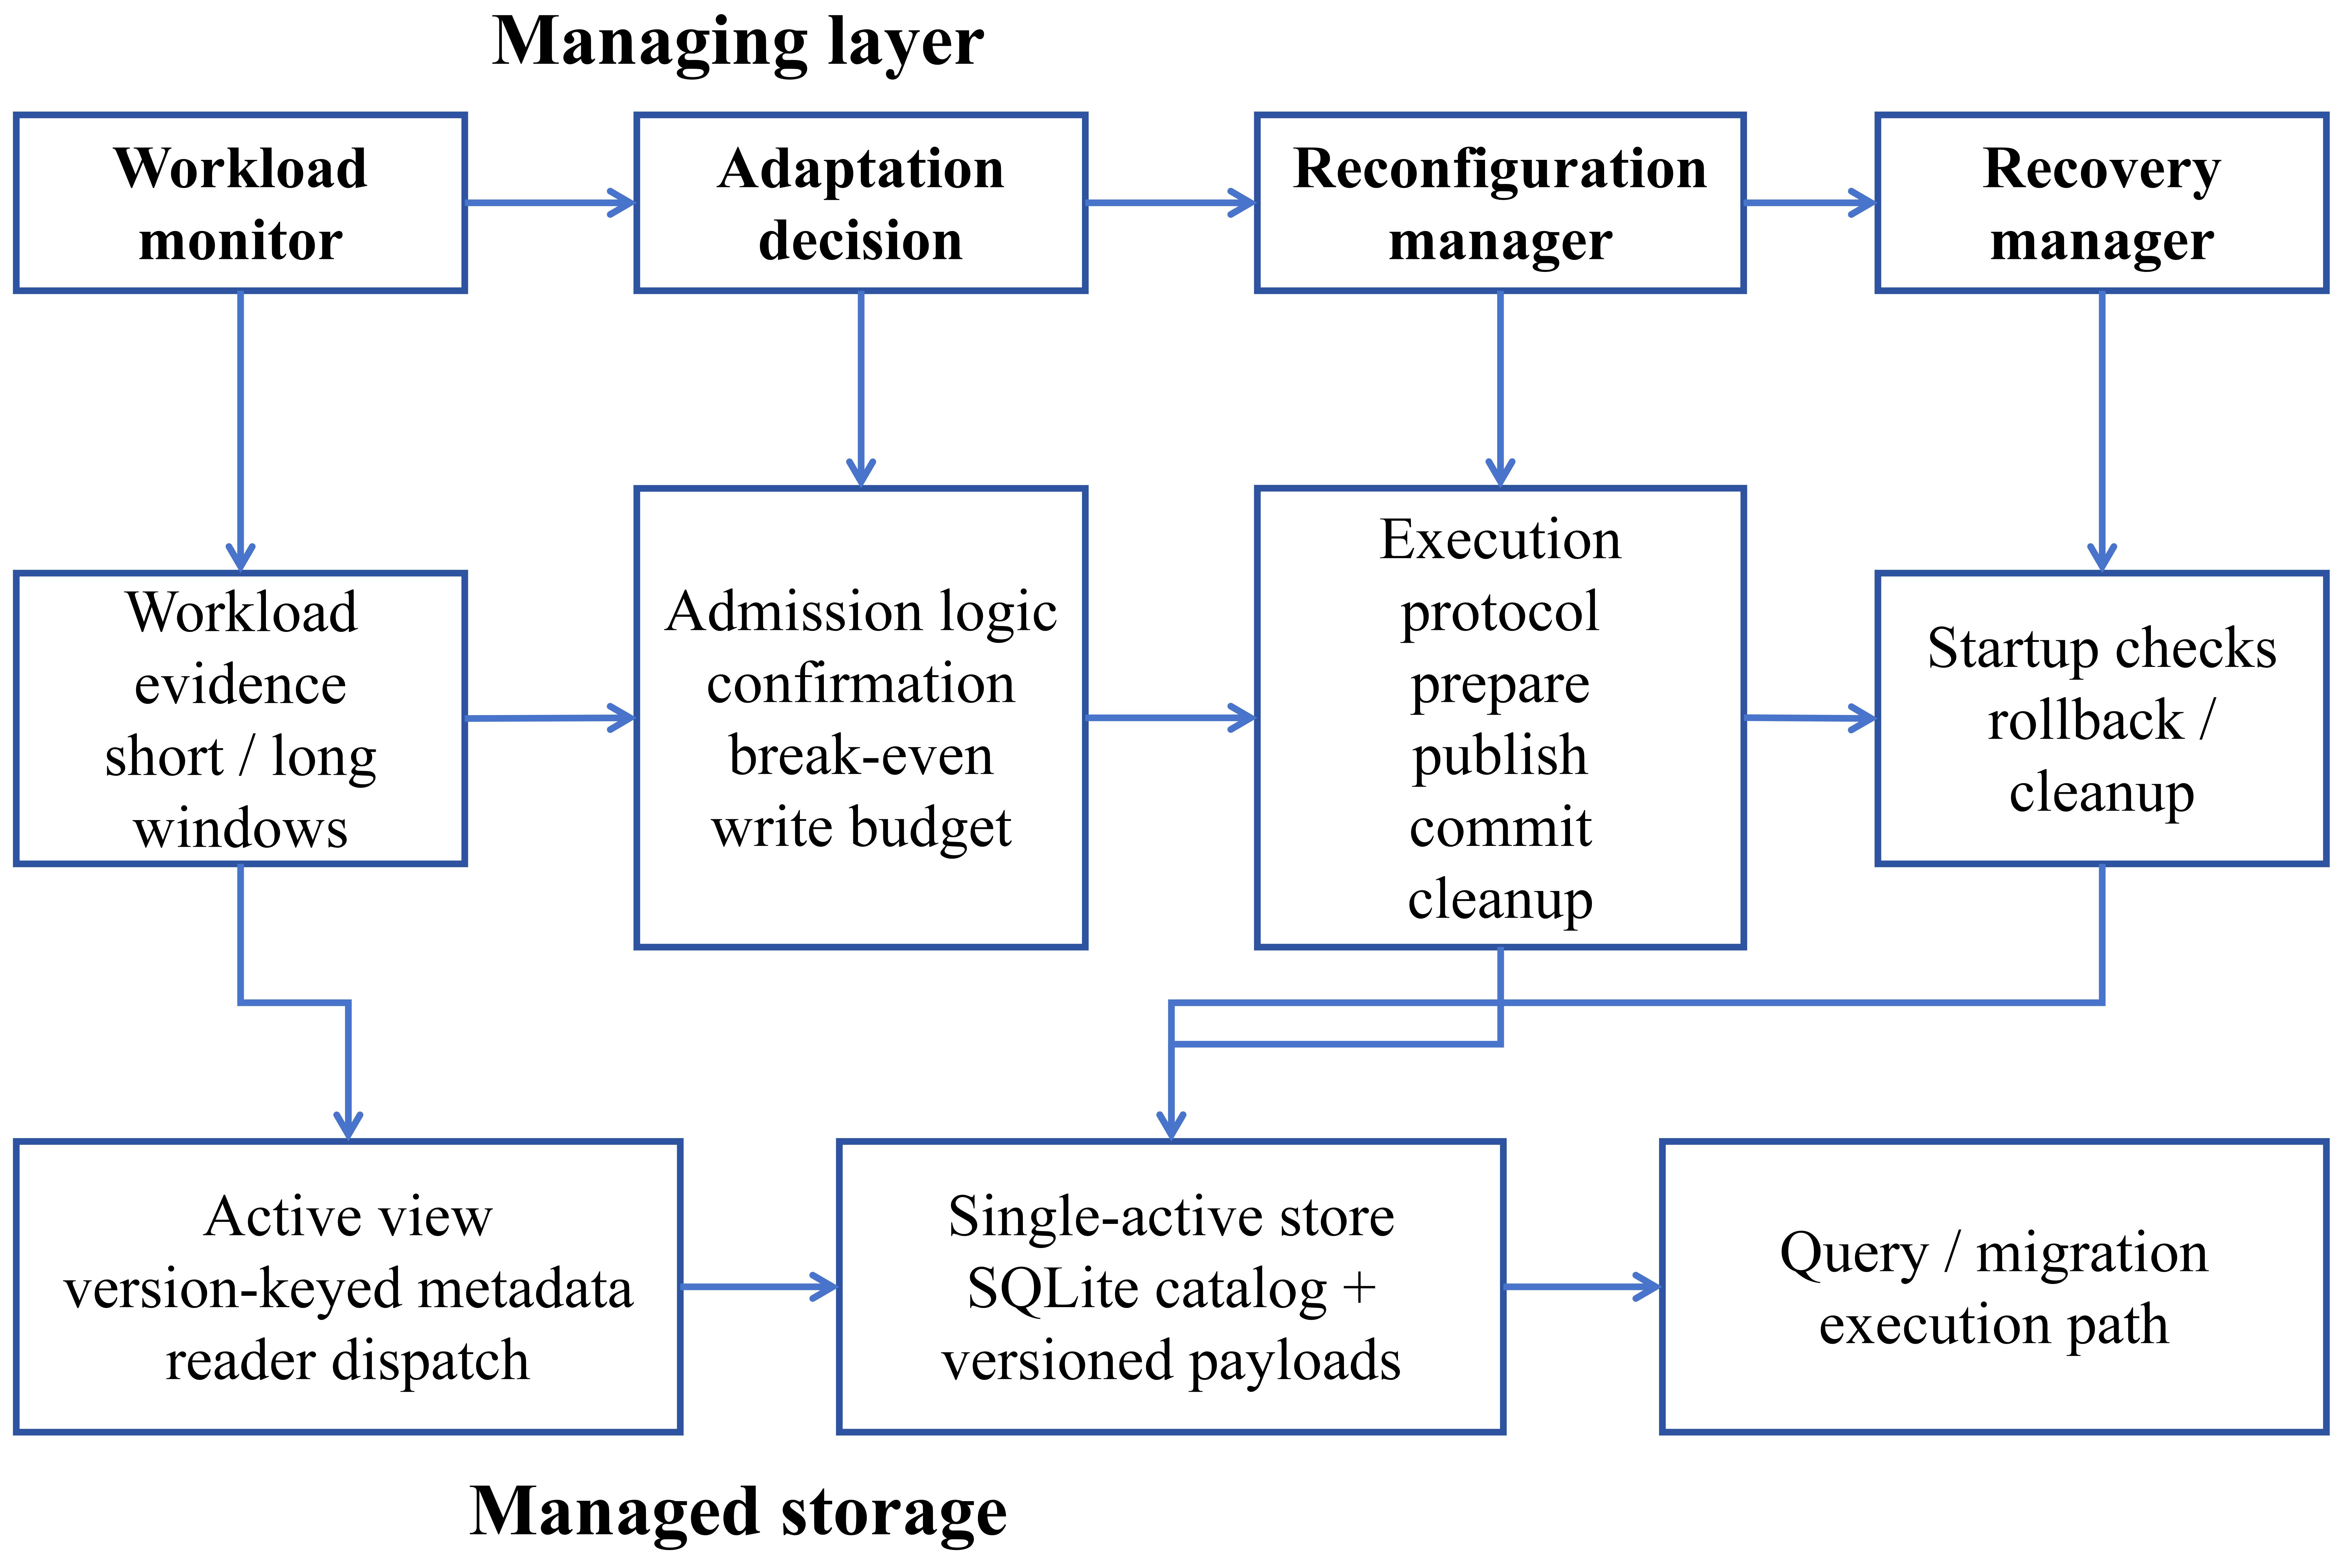
\includegraphics[width=0.68\textwidth]{Figure_1_architecture.png}
\caption{RePressDB runtime control path.}
\label{fig:architecture}
\end{figure*}

\section{Operational setting and research questions}
\label{sec:setting}

\subsection{Representations, queries, and information boundary}

RePressDB stores one-dimensional little-endian \texttt{float32} chunks. Five lossless representations are available. Two compress the whole chunk, using LZ4 or Zstandard level 3. The other three use LZ4 blocks of 64, 256, or 1,024 values. Whole-chunk formats keep metadata small and favor broad scans. Finer blocks avoid unrelated decompression during selective access.

The interface distinguishes eight query classes. They cover point lookup, three range lengths, three aggregate lengths, and threshold count. Calibration records file-backed median latency for every chunk, representation, and class. It also measures each directed source-to-target migration. The measured per-chunk tables are fixed before policy execution while the controller adapts to the observed query mix. The controller uses only past query events and the premeasured cost table; future trace duration and future migration time are unavailable at decision time.

For chunk $c$, representation $r$, and query class $q$, let $\ell_c(r,q)$ denote calibrated query cost. A directed migration $r\rightarrow r'$ has cost $m_c(r,r')$ and rewrite volume $b_c(r,r')$. For a trace of $T$ query events, measured-cost replay uses
\begin{equation}
C_{\mathrm{replay}}=
\sum_{t=1}^{T}\ell_{c_t}(r_{c_t,t},q_t)
+\sum_{e\in\mathcal{M}}m_{c_e}(r^-_e,r^+_e),
\label{eq:replay_cost}
\end{equation}
where $\mathcal{M}$ is the set of completed migrations. End-to-end execution instead records
\begin{equation}
T_{\mathrm{service}}=
T_{\mathrm{query\ path}}+T_{\mathrm{controller}}+T_{\mathrm{migration}},
\label{eq:e2e_cost}
\end{equation}
with the query path split into codec execution and catalog/dispatch time. Replay cost is used for controller comparisons, while file-backed service time is used for end-to-end execution. Throughout the paper, \emph{adaptation} denotes the controller-level decision process, \emph{reconfiguration} denotes an accepted layout change, and \emph{migration} denotes the physical rewrite that realizes the change.

\subsection{Architectural requirements}

\begin{table*}[t]
\centering
\caption{Architectural requirements and mechanisms.}
\label{tab:requirements}
\begin{tabularx}{\textwidth}{@{}p{0.15\textwidth}X X@{}}
\toprule
Requirement & Engineering concern & RePressDB mechanism \\
\midrule
Lossless service & Every query must return the same value before and after a layout change. & Independent truth arrays, raw checksums, target validation, and post-commit validation. \\
Single active version & Readers need an unambiguous visible representation. & One catalog active pointer; staging, published-pending, and previous files remain outside the active namespace. \\
Recoverable change & Interruption may occur between file and catalog operations. & Durable intent and state, fsynced encoded files, versioned publication, SQLite WAL commit, retained previous version, targeted recovery, and offline fsck. \\
Selective adaptation & Expensive rewrites require sustained workload evidence. & Dual windows, target agreement, repeated confirmation, gain threshold, directed break-even test, and cooldown. \\
Bounded write load & Many chunks can propose changes simultaneously. & Hard rewrite budget per global interval; denied proposals are recorded explicitly. \\
Controlled read overhead & Metadata and representation state should be reused across queries on one active version. & Version-keyed active-view cache with migration/recovery invalidation. \\
Diagnosability & Unexpected cost and interrupted change must be traceable. & Versioned manifests, decision and migration records, state-specific recovery reports, raw latency arrays, and SHA-256 checksums. \\
\bottomrule
\end{tabularx}
\end{table*}

\subsection{Research questions}

The evaluation is organized around three questions that follow the runtime control path from adaptation decision to physical execution and recovery.

\begin{table*}[t]
\centering
\caption{Research questions and evaluation evidence.}
\label{tab:rqs}
\footnotesize
\begin{tabularx}{\textwidth}{@{}p{0.055\textwidth}p{0.20\textwidth}p{0.31\textwidth}X@{}}
\toprule
RQ & Evaluated property & Primary measures & Main evidence \\
\midrule
RQ1 & Adaptation effectiveness and selectivity & Measured replay cost, completed migrations, unamortized and stale actions & Continuous multi-seed workloads, deployable baselines, and component ablations \\
RQ2 & Runtime efficiency of the implemented control path & Service time, catalog/dispatch work, throughput, p99 latency, calibration and startup cost & Paired active-view execution, logical-scale measurements, and foreground-interference campaigns \\
RQ3 & Dependability of physical reconfiguration & Active-version invariants, recovery completion, full-array equality, and query correctness & 600 protocol-boundary injections plus 500 randomized termination and corruption trials \\
\bottomrule
\end{tabularx}
\end{table*}

\section{Architecture and runtime behavior}
\label{sec:architecture}

\subsection{Dual-timescale monitor and admission chain}

Each chunk keeps the most recent 300 and 100 query classes. Monitoring begins immediately, but the policy waits for 200 local observations and evaluates the chunk every 100 local queries. For window $w$, empirical class weights $\widehat{p}_{c,w}(q)$ give
\begin{equation}
\widehat{L}_{c,w}(r)=
\sum_{q\in\mathcal{Q}}\widehat{p}_{c,w}(q)\ell_c(r,q).
\label{eq:window_cost}
\end{equation}
A target becomes eligible only when it minimizes \cref{eq:window_cost} in both windows. The controller then requires an 8\% relative improvement, three consecutive confirmations, and the directed break-even condition
\begin{equation}
1{,}200\,[\widehat{L}(r_{\mathrm{active}})-\widehat{L}(r^*)]
>1.25\,\widehat{m}_c(r_{\mathrm{active}},r^*).
\label{eq:break_even}
\end{equation}
A successful switch starts a 300-query cooldown. The global scheduler additionally enforces
\begin{equation}
\sum_{e\in\mathcal{M}_k} b_{c_e}(r^-_e,r^+_e)\le B_k
\label{eq:budget}
\end{equation}
for each 1,000-global-query interval $k$. The budget equals the largest measured directed rewrite in the corresponding measured cost table. A proposal that cannot fit is denied and counted.

\begin{table}[t]
\centering
\caption{Controller settings.}
\label{tab:parameters}
\begin{tabular}{@{}lr@{}}
\toprule
Setting & Value \\
\midrule
Long/short windows & 300 / 100 queries \\
Minimum observations & 200 queries \\
Decision interval & 100 queries \\
Required confirmations & 3 rounds \\
Cooldown & 300 queries \\
Projection horizon & 1,200 queries \\
Minimum relative gain & 8\% \\
Migration safety factor & 1.25 \\
Global budget interval & 1,000 queries \\
\bottomrule
\end{tabular}
\end{table}

\subsection{Single-active transaction and persistence assumptions}

Each chunk row records the current version and a retained previous version. It also stores the representation, file paths, sizes, checksum, migration state, pending target, and migration identifier.

A migration moves from \texttt{idle} through \texttt{intent}, \texttt{encoded}, \texttt{validated}, and \texttt{published}. Catalog commit places it in \texttt{committed\_pending\_cleanup}. Payload and metadata files are flushed and fsynced before validation, and publication uses same-volume \texttt{os.replace}. POSIX runs additionally fsync the containing directory. On the evaluated Windows/NTFS path, persistence uses flushed files, same-volume replacement, and SQLite WAL with \texttt{synchronous=FULL}.

Catalog commit defines the reader visibility boundary. It moves the old active fields into the previous-version fields and installs the validated target. The previous version remains retained until post-commit checksum and query validation complete, after which cleanup removes the retained files and returns the row to \texttt{idle}. \Cref{fig:reconfiguration_lifecycle} summarizes the state progression and the recovery obligations on either side of the visibility boundary.

\begin{figure*}[t]
\centering
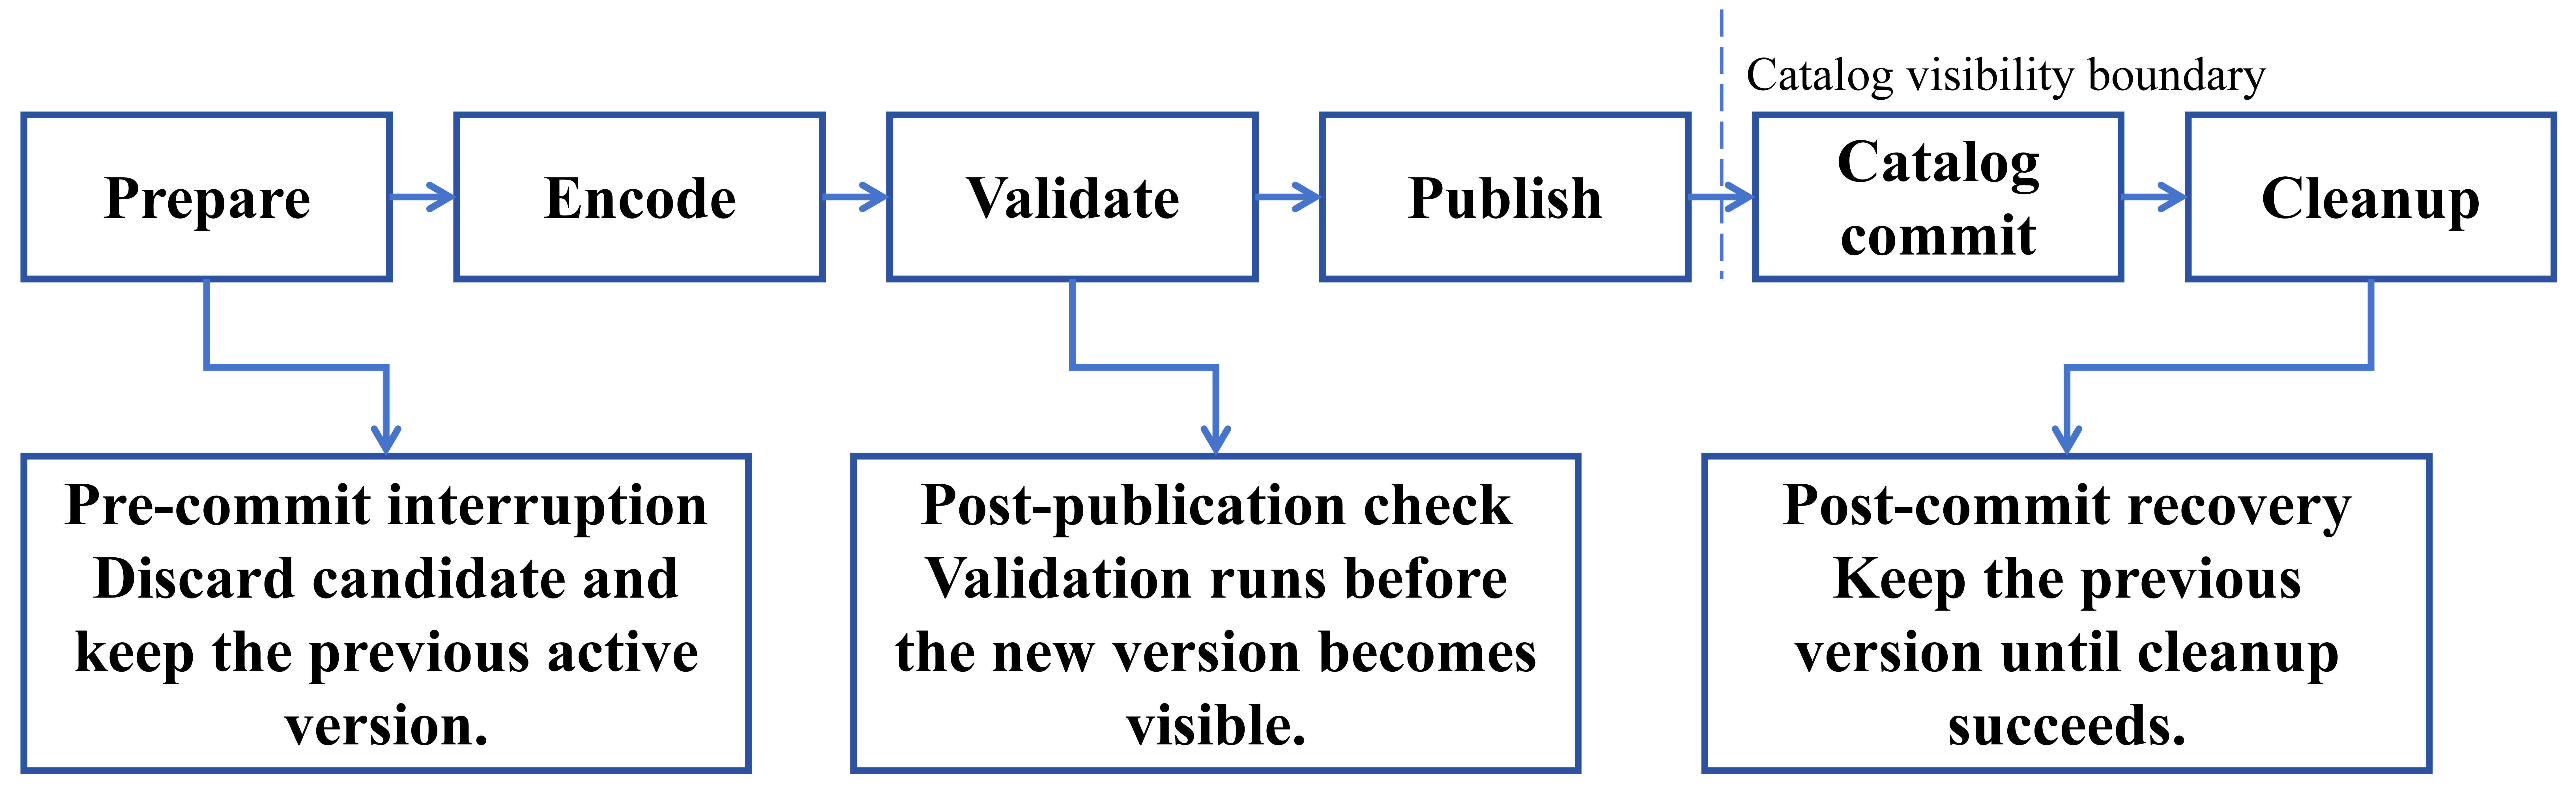
\includegraphics[width=0.96\textwidth]{Figure_2_reconfiguration_lifecycle.png}
\caption{Durable reconfiguration lifecycle.}
\label{fig:reconfiguration_lifecycle}
\end{figure*}

Three invariants guide recovery. Every catalog-visible active pointer names a complete checksum-validated version. At most one version is active. Startup reaches a valid idle state or raises an integrity error before serving queries.

\subsection{Recovery behavior}

Startup inspects non-idle catalog rows instead of scanning every payload file. Before catalog commit, the old version remains active and recovery removes the incomplete target. At \texttt{committed\_pending\_cleanup}, recovery validates the new active version. A valid target proceeds to cleanup. Otherwise the retained previous version is restored. Unreferenced staging and final files are removed. A separate offline fsck performs broader directory and checksum checks.

\subsection{Version-keyed active-view cache}

The active-view cache is keyed by $(\textit{chunk id},\textit{active version})$. An entry holds the resolved catalog row and its \texttt{StoredChunk}, together with parsed block metadata, the representation object, and open handles. A cache hit reaches codec execution directly. Commit, recovery, rollback, chunk creation, and store close invalidate the entry, so the first later query resolves a fresh view for the current version.

The active view makes version identity the consistency key for the steady-state read path. It also bounds metadata work: repeated queries on one active version reuse the resolved catalog and representation state. The paired implementation study evaluates this mechanism against an otherwise identical uncached read path while preserving the migration sequence in every pair.

\subsection{Concurrency isolation}

Readers use immutable versioned files. A process-local lock serializes active-view replacement and migration-state changes. Query workers maintain independent codec registries and file handles, and the migration writer uses its own codec state. This separation keeps mutable execution state within worker boundaries while active-version changes remain serialized through the store transaction.

\section{Evaluation design}
\label{sec:evaluation_design}

\subsection{Datasets and experimental roles}

PEMS04 and PEMS08 contain traffic sensor measurements sampled every five minutes \citep{song2020stsgcn}. Only PEMS04 is used for development. PEMS08 remains outside parameter selection. The Building Data Genome Project 2 (BDG2) provides energy-meter series from many buildings and meter types \citep{miller2020bdg2}. It supplies the cross-domain holdout and the physical-store experiments. Continuous replay also uses a disjoint BDG2 subset.

\begin{table*}[t]
\centering
\caption{Datasets and experimental roles.}
\label{tab:datasets}
\begin{tabularx}{\textwidth}{@{}p{0.13\textwidth}p{0.23\textwidth}p{0.23\textwidth}X@{}}
\toprule
Dataset/view & Source scale & Unit used & Role \\
\midrule
PEMS04 & 16,992 time points, 307 sensors, 3 channels & Sensor series and 2K/8K/16K chunks & Representation calibration, policy development, baseline selection, and controlled safeguards. \\
PEMS08 & 17,856 time points, 170 sensors, 3 channels & 32 held-out series; paired 8K/16K chunks & Independent traffic holdout. \\
BDG2 holdout & Public building-meter corpus & 32 held-out buildings; paired 8K/16K chunks & Cross-domain holdout. \\
BDG2 continuous replay & Disjoint building subset & 32 buildings for replay; eight pre-registered buildings for paired execution & Three phase-free trace families at two sizes. \\
BDG2 physical corpus & 3,053 candidate meter series & 564 eligible series, 720 8K chunks, 3,283 2K chunks & One million verified physical queries and 1,000 migrations. \\
BDG2 logical scale & 720 immutable physical templates & 32,768 to 327,680 logical chunks & Catalog, routing, startup, copy-on-write, and interference over shared physical templates. \\
\bottomrule
\end{tabularx}
\end{table*}

\subsection{Workloads and baselines}

Controlled traces contain clean stage changes, cyclic changes, stable regimes, and brief bursts. Continuous traces remove explicit boundaries: gradual-periodic drift changes query mixtures smoothly; mean-reverting drift repeatedly moves away from and back toward a baseline; noisy bursts combine finite deviations with background variation. Three seeds (20260801 to 20260803) are fixed before policy execution for each trace/size cell.

Deployable comparisons are initial-best, access-frequency hot/cold with deadband (AF-HC-D), Shape-EWMA-BE, Page-Hinkley with break-even (PH-BE), and RePressDB. Shape-EWMA-BE and PH-BE receive the same query classes and directed migration table as RePressDB; their configurations are selected on PEMS04 only. Best-static and a migration-aware hindsight oracle use future information and serve as offline references.

\subsection{End-to-end pairing and timing}

The formal end-to-end campaign uses eight pre-registered BDG2 buildings. It crosses three traces with two chunk sizes, three repetitions, and three policies. Each of the 54 policy cells runs once through an uncached read path and once through the version-keyed active-view path, producing \EndToEndWorkers{} isolated workers.

Implementation order is balanced 27/27, and policy order is cyclically balanced. Every worker starts from an independent copy of the same base store. One verification query per chunk prewarms the active view outside the timed interval; a reload caused by migration remains inside it. Workers run sequentially in isolated processes, so runtime library and store state are released between cells. Every measured query is checked against an independent \texttt{float32} truth array. Timing separates query execution, controller work, and migration, using \texttt{time.perf\_counter\_ns}.

\subsection{Environment and reproducibility}

The evaluation host runs Microsoft Windows 11 Home (build 26200) on NTFS, with an Intel Core i7-14700HX, 16.87 GB of visible memory, and a 1.024 TB NVMe SSD. Experiments use Python 3.10.20, and SQLite runs in WAL mode with \texttt{synchronous=FULL}. Absolute service times depend on the host, so end-to-end comparisons use balanced within-pair ratios. Package versions, hardware identifiers, script hashes, trace manifests, result files, and generation code are recorded in the artifact and Supplementary Material.

\subsection{Statistical treatment}

For multi-seed replay, one trace realization at one trace/size setting is the statistical unit, giving 18 units. Ratios are equal-weight geometric means. For end-to-end execution, one trace/size/repeat cell is the paired unit, again giving 18 units per policy. We report geometric-mean ratios, percentile-bootstrap 95\% intervals from 20,000 resamples, medians, and win counts. Buildings sharing one trace remain within the same paired unit.

\section{Results}
\label{sec:results}

\subsection{RQ1: Adaptation effectiveness under nonstationary workloads}

Across the 18 continuous trace realizations, RePressDB has lower measured replay cost than Shape-EWMA-BE in every cell. The aggregate ratio is \ReplayRepressShapeRatio, and completed migrations fall from \ReplayShapeMigrations{} to \ReplayRepressMigrations, a 48.75\% reduction. We first establish the layout opportunity and then examine adaptation under continuous workload change and the contribution of the admission rules.

\paragraph{Physical-layout opportunity}
Across PEMS04, PEMS08, and BDG2, the preferred representation changes with query shape. Whole-chunk compression frequently serves broad scans best, while 64- or 256-value blocks frequently favor point, short-range, and selective aggregate queries. These measured differences establish the runtime opportunity used by the controller when evaluating a reconfiguration.

\paragraph{Continuous nonstationarity}
\begin{figure*}[!tbp]
\centering
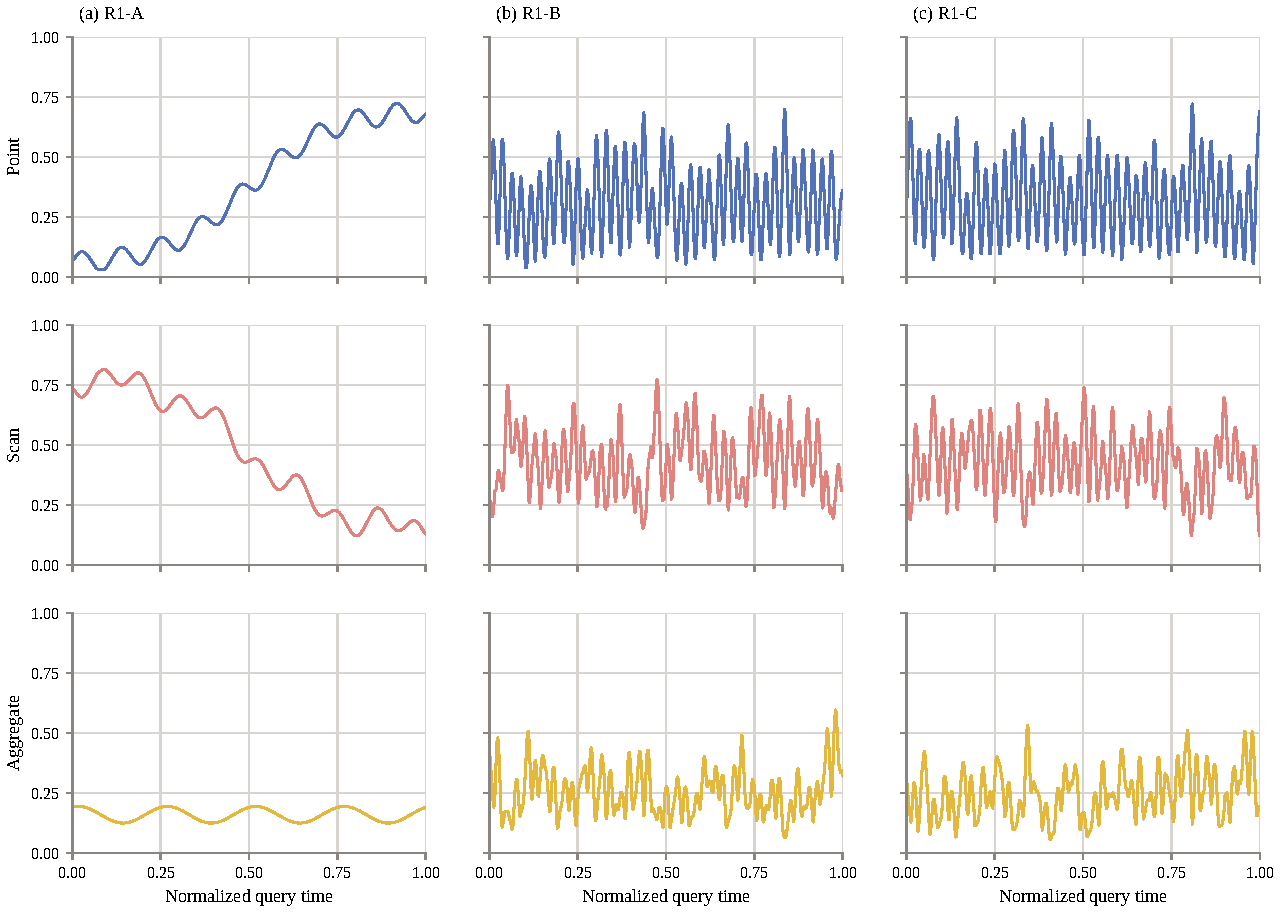
\includegraphics[width=0.84\textwidth]{Figure_2_continuous_traces.pdf}
\caption{Continuous nonstationary query mixtures.}
\label{fig:continuous_traces}
\end{figure*}

\begin{table*}[!tbp]
\centering
\caption{Multi-seed replay results.}
\label{tab:multiseed_cost}
\begin{threeparttable}
\begin{tabular}{@{}lrrrrrr@{}}
\toprule
Trace & Size & RePress/Shape & RePress/initial & RePress/PH-BE & RePress mig. & Shape mig. \\
\midrule
Gradual--periodic & 8K & 0.9453 & 0.9453 & 0.9590 & 44 & 0 \\
Gradual--periodic & 16K & 0.9586 & 0.9067 & 0.9956 & 55 & 40 \\
Mean-reverting & 8K & 0.9806 & 0.9806 & 1.0008 & 6 & 0 \\
Mean-reverting & 16K & 0.9541 & 0.9355 & 0.9624 & 41 & 170 \\
Noisy bursts & 8K & 0.9795 & 0.9795 & 0.9986 & 6 & 0 \\
Noisy bursts & 16K & 0.9527 & 0.9472 & 0.9648 & 33 & 151 \\
\midrule
All cells & -- & 0.9617 & 0.9488 & 0.9800 & 185 & 361 \\
\bottomrule
\end{tabular}
\begin{tablenotes}[flushleft]\footnotesize
\item PH-BE denotes the Page--Hinkley break-even baseline configured on PEMS04. Ratios below one favor RePressDB. File-backed service time is evaluated separately in RQ2.
\end{tablenotes}
\end{threeparttable}
\end{table*}


The aggregate RePressDB/Shape-EWMA-BE replay ratio is \ReplayRepressShapeRatio{} (bootstrap 95\% CI \ReplayRepressShapeLow--\ReplayRepressShapeHigh). Ratios to initial-best, PH-BE, AF-HC-D, and free hindsight best-static are \ReplayRepressInitialRatio, \ReplayRepressPHRatio, \ReplayRepressAFHCRatio, and \ReplayRepressBestStaticRatio. Best-static has complete-trace knowledge and a free initial choice, so it serves as an optimistic offline reference.

\begin{figure}[!htbp]
\centering
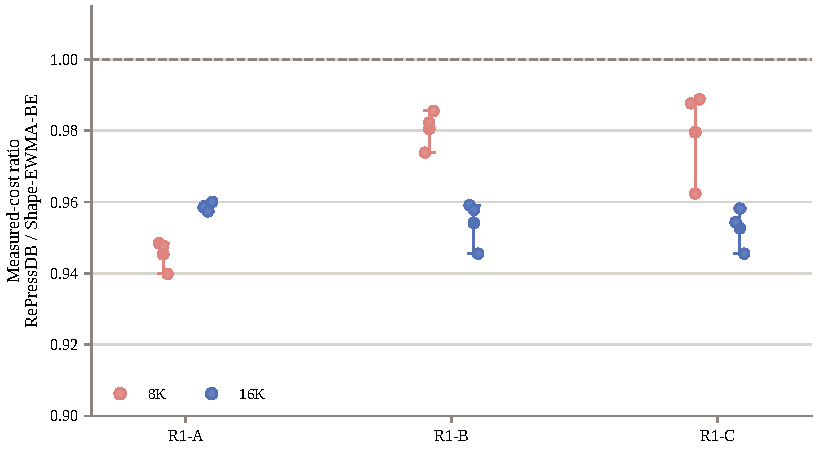
\includegraphics[width=0.98\columnwidth]{Figure_4_multiseed_total_cost.pdf}
\caption{Multi-seed measured-cost ratios.}
\label{fig:multiseed_cost}
\end{figure}

\begin{figure*}[!b]
\centering
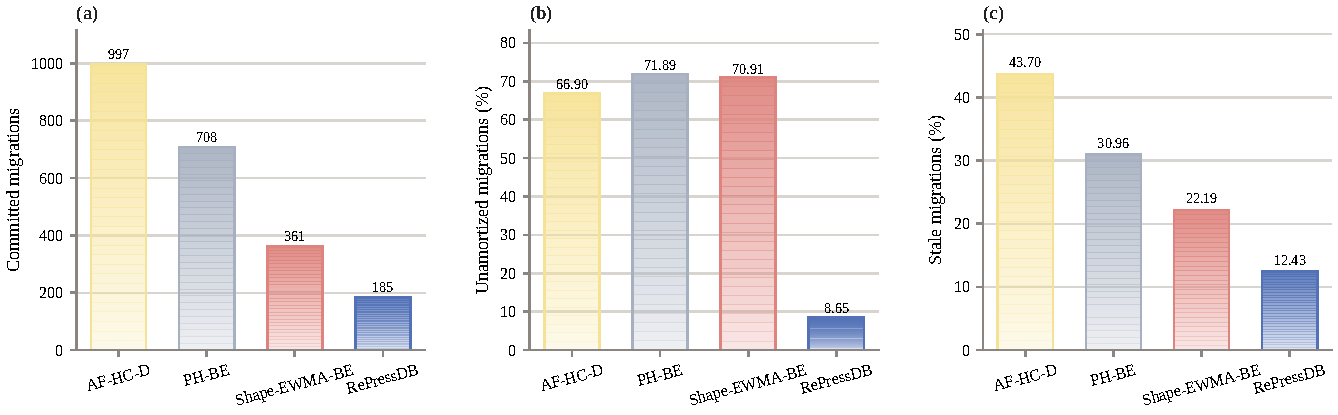
\includegraphics[width=0.80\textwidth]{Figure_5_multiseed_migration_risk.pdf}
\caption{Multi-seed migration behavior.}
\label{fig:migration_risk}
\end{figure*}


Migration activity differs more strongly among the adaptive policies than aggregate replay cost. RePressDB executes \ReplayRepressMigrations{} migrations versus \ReplayShapeMigrations{} for Shape-EWMA-BE, a 48.75\% reduction. Unamortized rates are \ReplayRepressUnamortized{} and \ReplayShapeUnamortized{}, while stale rates are \ReplayRepressStale{} and \ReplayShapeStale{}. PH-BE has an aggregate RePressDB/PH-BE ratio of \ReplayRepressPHRatio, with RePressDB lower in 15 of 18 cells.


\paragraph{Admission selectivity}
\begin{table*}[!tbp]
\centering
\caption{Ablation results.}
\label{tab:unified_ablation}
\begin{tabular}{@{}lrrrrr@{}}
\toprule
Variant & Cost ratio & 95\% CI & Migrations & Median unamortized & Median stale \\
\midrule
Full RePressDB & 1.0000 & [1.0000, 1.0000] & 66 & 3.33\% & 2.78\% \\
No break-even & 0.9667 & [0.9428, 0.9886] & 130 & 16.23\% & 16.23\% \\
No confirmation & 0.9857 & [0.9600, 1.0102] & 229 & 10.51\% & 0.00\% \\
No cooldown & 1.0000 & [1.0000, 1.0000] & 66 & 3.33\% & 2.78\% \\
No write budget & 0.9994 & [0.9988, 0.9999] & 66 & 3.33\% & 2.78\% \\
Short-window only & 0.9941 & [0.9803, 1.0073] & 126 & 8.33\% & 2.63\% \\
\bottomrule
\end{tabular}
\end{table*}


The largest changes in migration activity occur when break-even or repeated confirmation is removed. Without break-even, the replay-cost ratio is 0.9667, migrations rise from 66 to 130, and the median unamortized rate rises from 3.33\% to 16.23\%. Removing confirmation produces 229 migrations at a cost ratio of 0.9857. Using the short window alone produces 126 migrations at a cost ratio of 0.9941. In these cells, cooldown and the write-budget constraint seldom alter aggregate replay values; they continue to cap rapid reversals and total rewrite activity.

The clean-stage holdout, reported in the Supplementary Material, characterizes the responsiveness trade-off. Shape-EWMA-BE reacts earlier to clear persistent phase changes; RePressDB performs fewer migrations and rewrites fewer bytes over the same traces.

\paragraph{RQ1 summary}
Across continuous nonstationary workloads, RePressDB combines lower measured replay cost with fewer persistent reconfigurations than the principal reactive baseline. The ablation associates this selectivity most strongly with persistence checks and migration-aware admission.

\subsection{RQ2: End-to-end runtime behavior}

With the version-keyed active view, the paired file-backed campaign executes \EndToEndQueries{} measured queries, each verified against an independent truth array, and gives a RePressDB/Shape-EWMA-BE service-time ratio of \EndToEndRepressShapeRatio. The paired ablation isolates metadata-resolution cost, while the scale and interference studies examine supporting runtime mechanisms.

\begin{figure*}[!t]
\centering
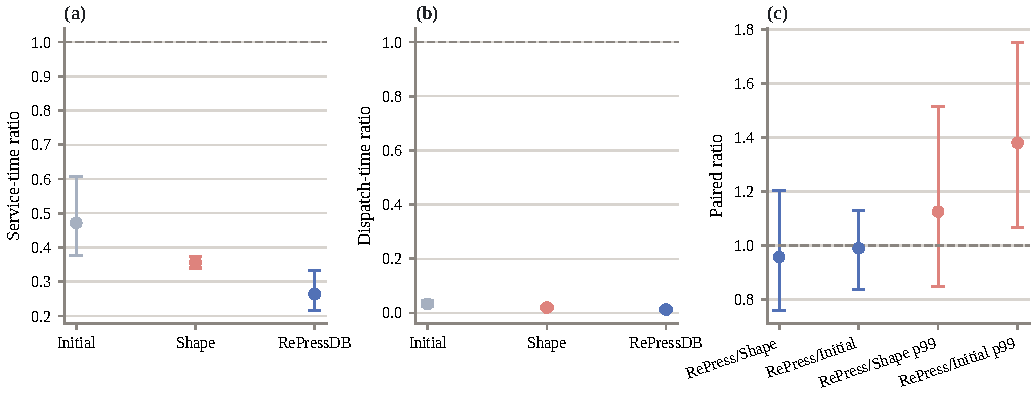
\includegraphics[width=0.80\textwidth]{Figure_9_active_view_end_to_end.pdf}
\caption{Active-view and end-to-end comparison.}
\label{fig:e2e_active_view}
\end{figure*}

\paragraph{Policy-level service time}
The RePressDB/Shape-EWMA-BE ratio is \EndToEndRepressShapeRatio{} (95\% CI \EndToEndRepressShapeLow--\EndToEndRepressShapeHigh), with median \EndToEndRepressShapeMedian; each policy is faster in nine of 18 paired units. RePressDB/initial-best is \EndToEndRepressInitialRatio{} (95\% CI \EndToEndRepressInitialLow--\EndToEndRepressInitialHigh). The corresponding p99 ratios are \EndToEndRepressShapePnnRatio{} and \EndToEndRepressInitialPnnRatio, respectively. These measurements place aggregate service time close across the compared policies, while tail latency reflects the timing of controller and migration activity.

\paragraph{Active-view execution}
The paired read-path ablation compares the version-keyed active view with an otherwise identical uncached path. Across 8,454,033 queries per implementation, the uncached path performs 16,909,113 catalog-row loads and 2,358,417 metadata parses, compared with 246 of each on the active-view path. Active-view/uncached service-time ratios are \CacheInitialServiceRatio{} for initial-best, \CacheShapeServiceRatio{} for Shape-EWMA-BE, and \CacheRepressServiceRatio{} for RePressDB. The corresponding dispatch reductions are 96.71\%, 98.02\%, and 98.77\%. Every paired run preserves the same migration signature, including event index, chunk, source and target codec, and rewrite bytes.


\paragraph{Calibration, scale, and foreground interference}
Fresh calibration covers 64 chunks, five codecs, eight query classes, and 25 source-to-target entries per chunk. The run takes \CalibrationSeconds{} s, reads \CalibrationReadMB{} MB, and writes \CalibrationWriteMB{} MB. The full cleaned-BDG2 store contains 564 eligible series and completes one million verified queries plus 1,000 migrations. Logical replication reaches 32,768, 163,840, and 327,680 chunks, corresponding to 1, 5, and 10 GiB logical raw sizes. Catalog overhead remains near 300 bytes per logical chunk, with clean-startup medians of 0.283 s, 2.656 s, and 5.526 s.

Calibration sensitivity is detailed in the Supplementary Material. Replacing chunk-specific tables with a sampled population profile raises replay cost by 8.35--9.38\%. Independent perturbations of up to $\pm20$\% in individual entries change aggregate true cost only slightly, indicating that local measurement error has a smaller effect than removing chunk-specific structure.

Foreground interference is measured with bursts of 50 background copy-on-write migrations. Across 54 counterbalanced pairs, the foreground-throughput ratio is 0.9764 (95\% CI 0.9741--0.9786) and p99 amplification is 1.0569 (95\% CI 1.0492--1.0645). All 5.4 million measured queries and 2,700 migrations satisfy the query-correctness checks.

\begin{figure*}[!t]
\centering
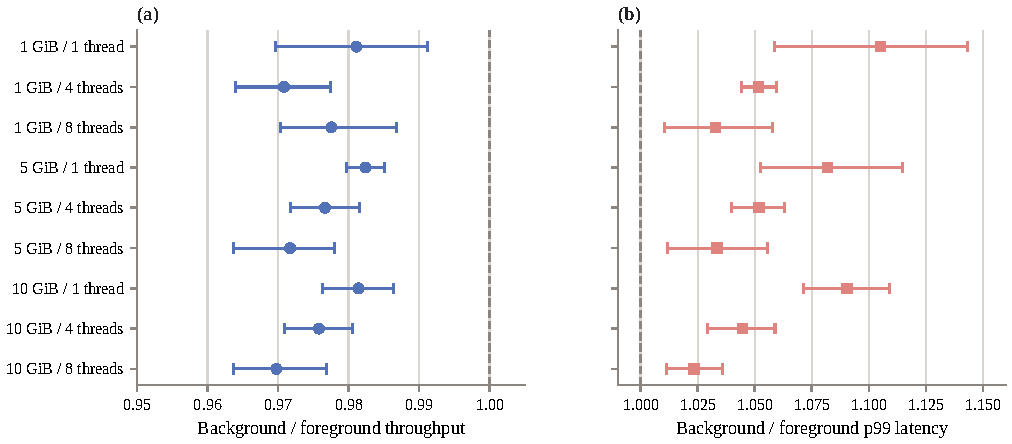
\includegraphics[width=0.86\textwidth]{Figure_8_interference_core.pdf}
\caption{Foreground interference under background migration.}
\label{fig:interference}
\end{figure*}

\paragraph{RQ2 summary}
The implemented control path delivers aggregate service time close to the comparison policies, and the active view removes most repeated catalog and metadata work. Calibration, catalog scaling, and bounded migration bursts add modest overhead in the measured settings.

\FloatBarrier
\subsection{RQ3: Dependable reconfiguration}

The recovery campaign combines deterministic boundary injections with randomized interruption and corruption. The boundary campaign completes 100,000 verified file queries, 1,000 migrations, and 600 controlled exceptions across six migration states. A second campaign adds 500 trials covering abrupt process termination, post-commit payload truncation, post-commit metadata corruption, and orphan files.

\begin{table}[H]
\centering
\caption{Recovery campaign summary.}
\label{tab:recovery_campaign}
\scriptsize
\begin{tabularx}{\columnwidth}{@{}p{0.35\columnwidth}rX@{}}
\toprule
Trial class & Trials & Verified condition \\
\midrule
Protocol-boundary interruption & 600 & Active-store invariants and verified queries \\
Abrupt process termination & 300 & Idle catalog, one active payload, full-array equality, 20 spot queries \\
Payload truncation & 75 & Valid active version; integrity and full-array checks \\
Metadata corruption & 50 & Valid active version; integrity and full-array checks \\
Orphan files & 75 & Valid active catalog; cleanup and query checks \\
\midrule
Total & \CombinedRecoveryTrials{} & Valid active-store state for every completed trial \\
\bottomrule
\end{tabularx}
\end{table}

Randomized termination reaches every protocol state from \texttt{idle} through \texttt{committed\_pending\_cleanup}. All randomized trials recover to a valid idle catalog with one active payload, no temporary files, full-array equality, and 20 correct spot queries. Detailed state counts and recovery checks appear in the Supplementary Material.

\paragraph{RQ3 summary}
The single-active transaction preserves a valid published representation across the tested interruption and corruption scenarios. Recovery returns all \CombinedRecoveryTrials{} completed trials to a query-correct active-store state within the evaluated fault model.

\FloatBarrier

\section{Discussion}
\label{sec:discussion}

\subsection{Architectural implications of durable self-adaptation}

RePressDB links two forms of runtime state: the evidence used to admit an adaptation and the durable state changed by the resulting reconfiguration. Workload persistence and rewrite economics govern admission; versioned publication and recovery govern execution. The catalog-visible active version connects these concerns, giving the controller and storage layer a shared reference for action cost, reader visibility, and recovery state.

The evaluation mirrors this separation. RQ1 studies adaptation choices under common measured costs, RQ2 measures the realized read and migration path, and RQ3 exercises the durable state transitions. This structure makes the consequences of an accepted adaptation visible at both policy and implementation levels.

\subsection{Balancing responsiveness and reconfiguration cost}

Adaptation frequency is itself an operational concern in self-adaptive systems: frequent or poorly converging actions can increase overhead and disturb the managed system \citep{salama2017stability,ayala2021prodspl}. The RePressDB ablation shows the same tension for persistent storage changes. Removing confirmation or break-even can lower replay cost in some cells, yet it also increases the number of migrations and the fraction that fail to amortize within the evaluation horizon.

Cooldown and the global write budget provide separate controls over actuation. Their aggregate effect is small in the reported ablation cells because those traces seldom drive the constraints strongly. They still define limits on rapid reversals and concurrent rewrite demand, which becomes relevant when many chunks propose reconfiguration at the same time.

\subsection{Aligning adaptation models with execution boundaries}

The active-view ablation shows that a runtime cost model depends on the implementation path that realizes it. Calibration assumes parsed metadata and representation state are already available; repeated catalog resolution and metadata reconstruction add work outside that measured path. Binding resolved state to the active version restores a stable correspondence between calibrated query cost and steady-state execution.

This issue extends beyond the layouts used here. Cost-aware adaptation needs a consistent unit of execution. Cache state, metadata resolution, worker isolation, and publication semantics can therefore influence the validity of a cost model even when they do not appear in the policy equation. Treating these mechanisms as part of the runtime architecture helps keep decision models and executed actions aligned.

\subsection{Deployment considerations}

RePressDB fits deployments where representation choice materially affects query work, workload regimes persist long enough to amortize a rewrite, and the storage layer can retain a previous version through publication and validation. The current implementation uses per-chunk calibration; substantial changes in hardware, codec configuration, or cache policy should therefore be accompanied by a refreshed cost table. Feature-conditioned cost prediction could reduce calibration work while retaining the same admission and recovery structure.

Very short-lived regime changes leave little time for a physical rewrite to recover its cost and may be better served by routing or scheduling mechanisms. RePressDB is most applicable when adaptation has durable consequences and the service needs explicit control over the frequency, cost, and recovery of those consequences.

\section{Threats to validity}
\label{sec:threats}

\subsection{Construct validity}

Measured-cost replay uses per-class latency profiles and directed migration costs to compare controller decisions under a common cost basis. The paired file-backed campaign supplies the query path, catalog work, controller time, and migration time used for end-to-end service comparisons. The uncached read path is treated as an architectural ablation of metadata resolution. Best-static and the migration-aware hindsight oracle use future trace information and serve only as offline references. Stale and unamortized classifications use fixed operational horizons throughout the study.

\subsection{Internal and conclusion validity}

All parameter development uses PEMS04. PEMS08 and BDG2 holdouts, multi-seed traces, fault injection, calibration sensitivity, and end-to-end execution remain outside parameter selection. A trace realization is the replay unit; a trace/size/repeat cell is the paired unit for end-to-end analysis, with buildings sharing one trace kept in the same unit. Equal-weight geometric means are reported with confidence intervals, medians, and win counts, and observed timing outliers remain in the analysis.

\subsection{External validity}

The evaluation combines real traffic and building-meter values with controlled or semi-synthetic query flows. Five LZ4/Zstandard layouts define the representation space, and the paired file-backed campaign runs on one Windows/NTFS host. Replication on additional storage stacks, cache regimes, and representation families would broaden the empirical coverage. The logical-scale experiment measures catalog, routing, startup, copy-on-write, and interference over shared immutable physical templates.

\subsection{Fault-model validity}

The recovery campaign targets software-visible interruption and corruption modes: named migration states, abrupt child-process termination, payload truncation, metadata corruption, and orphan files. POSIX runs additionally fsync the containing directory; the evaluated Windows path uses flushed files, same-volume replacement, and SQLite WAL with \texttt{synchronous=FULL}. Hardware power interruption, storage-controller write reordering, and system-call-level crash injection require a stronger durability test environment and are outside the fault model evaluated here.

\section{Related work}
\label{sec:related_work}

\subsection{Self-adaptive architecture and physical design}

Autonomic and self-adaptive systems organize runtime change around monitoring, analysis, planning, execution, and shared knowledge \citep{kephart2003vision,salehie2009landscape}. Architecture-based approaches such as Rainbow connect runtime decisions to explicit system models and reusable effectors \citep{garlan2004rainbow}, while later roadmaps emphasize uncertainty, assurance, and evaluation of the complete feedback loop \citep{delemos2013roadmap,krupitzer2015survey}.

Work on adaptation quality provides a closer point of comparison. Architectural-stability analysis treats adaptation frequency, settling behavior, and overhead as properties of runtime adaptation \citep{salama2017stability}. ProDSPL uses proactive control to reduce reconfiguration frequency while maintaining system utility \citep{ayala2021prodspl}. ML2ASR+ reduces the adaptation space before runtime analysis \citep{quin2022adaptationspace}, and uncertainty-aware proactive control combines prediction quality with adaptation latency and decision cost \citep{chen2024reliable}. These studies frame runtime adaptation in terms of stability, action frequency, analysis cost, and uncertainty. In RePressDB, the managed action is a persistent storage rewrite with explicit publication and recovery state.

Database physical design supplies the complementary storage perspective. Cost-driven index selection and automatic tuning choose database structures from workload evidence \citep{chaudhuri1997autoadmin,bruno2005physical}; database cracking brings reorganization into query execution \citep{idreos2007cracking}; and self-driving systems tune broader configurations or forecast workloads \citep{vanaken2017ottertune,pavlo2017selfdriving,li2026forecasting}. Concept-drift methods provide mechanisms for adapting to time-varying observations \citep{gama2014drift,bifet2007adwin}. RePressDB connects these decision mechanisms to a physical-layout actuator whose rewrite cost, write budget, publication state, and recovery path are represented explicitly in the runtime architecture.

\subsection{Compressed time-series storage and recovery}

Column stores integrate compression with execution because representation and operator cost interact directly \citep{stonebraker2005cstore,abadi2006compression}. MorphStore extends compression-aware execution \citep{damme2020morphstore}; Gorilla, BTrDB, and Sprintz illustrate specialized time-series representations \citep{pelkonen2015gorilla,andersen2016btrdb,blalock2018sprintz}. RePressDB uses representation diversity as the adaptation space and studies replacement of the active layout after deployment as the workload evolves.

Write-ahead logging, versioned state, and recovery protocols provide established foundations for durable systems \citep{mohan1992aries,gray1992transaction,sqlitewal}. Dependability terminology distinguishes prevention, tolerance, removal, and forecasting \citep{avizienis2004dependability}. RePressDB applies these foundations to runtime physical reconfiguration: the same catalog transition that publishes a new representation also defines the recovery state observed after interruption.

\section{Conclusion}
\label{sec:conclusion}

RePressDB combines workload-aware adaptation with recoverable physical-layout reconfiguration for nonstationary time-series services. The controller uses short- and long-term query evidence, measured layout cost, directed rewrite economics, and bounded actuation to admit representation changes. Accepted changes pass through versioned single-active publication, and the active view keeps steady-state readers aligned with the catalog version used by the recovery protocol.

Across 18 continuous trace realizations, the measured-cost ratio relative to Shape-EWMA-BE is \ReplayRepressShapeRatio{}, with migrations reduced from \ReplayShapeMigrations{} to \ReplayRepressMigrations. The paired file-backed campaign reports a RePressDB/Shape-EWMA-BE service-time ratio of \EndToEndRepressShapeRatio{} over \EndToEndQueries{} verified queries. All \CombinedRecoveryTrials{} completed interruption and corruption trials recover to a valid active-store state with correct query results. These results support a design principle for self-adaptive storage: when adaptation changes durable state, the decision model, action cost, publication state, and recovery path benefit from a shared runtime control structure.

\section*{CRediT authorship contribution statement}

\textbf{Zhichao Zhang}: Conceptualization; Methodology; Software; Formal analysis; Investigation; Validation; Data curation; Visualization; Project administration; Supervision; Writing -- original draft; Writing -- review and editing. \textbf{Xiaolu Peng}: Software; Investigation; Validation; Data curation; Resources; Writing -- review and editing. \textbf{Daoqi Sun}: Formal analysis; Investigation; Validation; Visualization; Writing -- review and editing.

\section*{Data and artifact availability}

PEMS04, PEMS08, and the Building Data Genome Project 2 remain available from their cited sources. RePressDB source code, archived summaries, manifests, and generation scripts are provided at \href{\ArtifactRepositoryURL}{\ArtifactRepositoryURLText}. Versioned result archives, including raw end-to-end latency arrays, are distributed through \href{\ArtifactReleaseURL}{\ArtifactReleaseURLText}. Numerical macros and the principal result tables are generated directly from archived evidence files.

\section*{Declaration of competing interest}

The authors declare that they have no known competing financial interests or personal relationships that could have appeared to influence the work reported in this paper.

\section*{Funding}

This research received no specific grant from funding agencies in the public, commercial, or not-for-profit sectors.

\section*{Acknowledgements}

The authors acknowledge the maintainers of the public PEMS and Building Data Genome Project 2 datasets.


\balance
\bibliographystyle{elsarticle-harv}
\bibliography{references}

\end{document}
